\documentclass{article}
\usepackage[dvipnames, table]{xcolor}
\usepackage[utf8]{inputenc}
\usepackage[dutch]{babel}
\usepackage{tabularx}
\usepackage{pdfpages}
\usepackage{enumitem}
\usepackage{geometry}
\geometry{
	a4paper,
	total={170mm,257mm},
	left=27mm,
	top=20mm,
}

\begin{document}
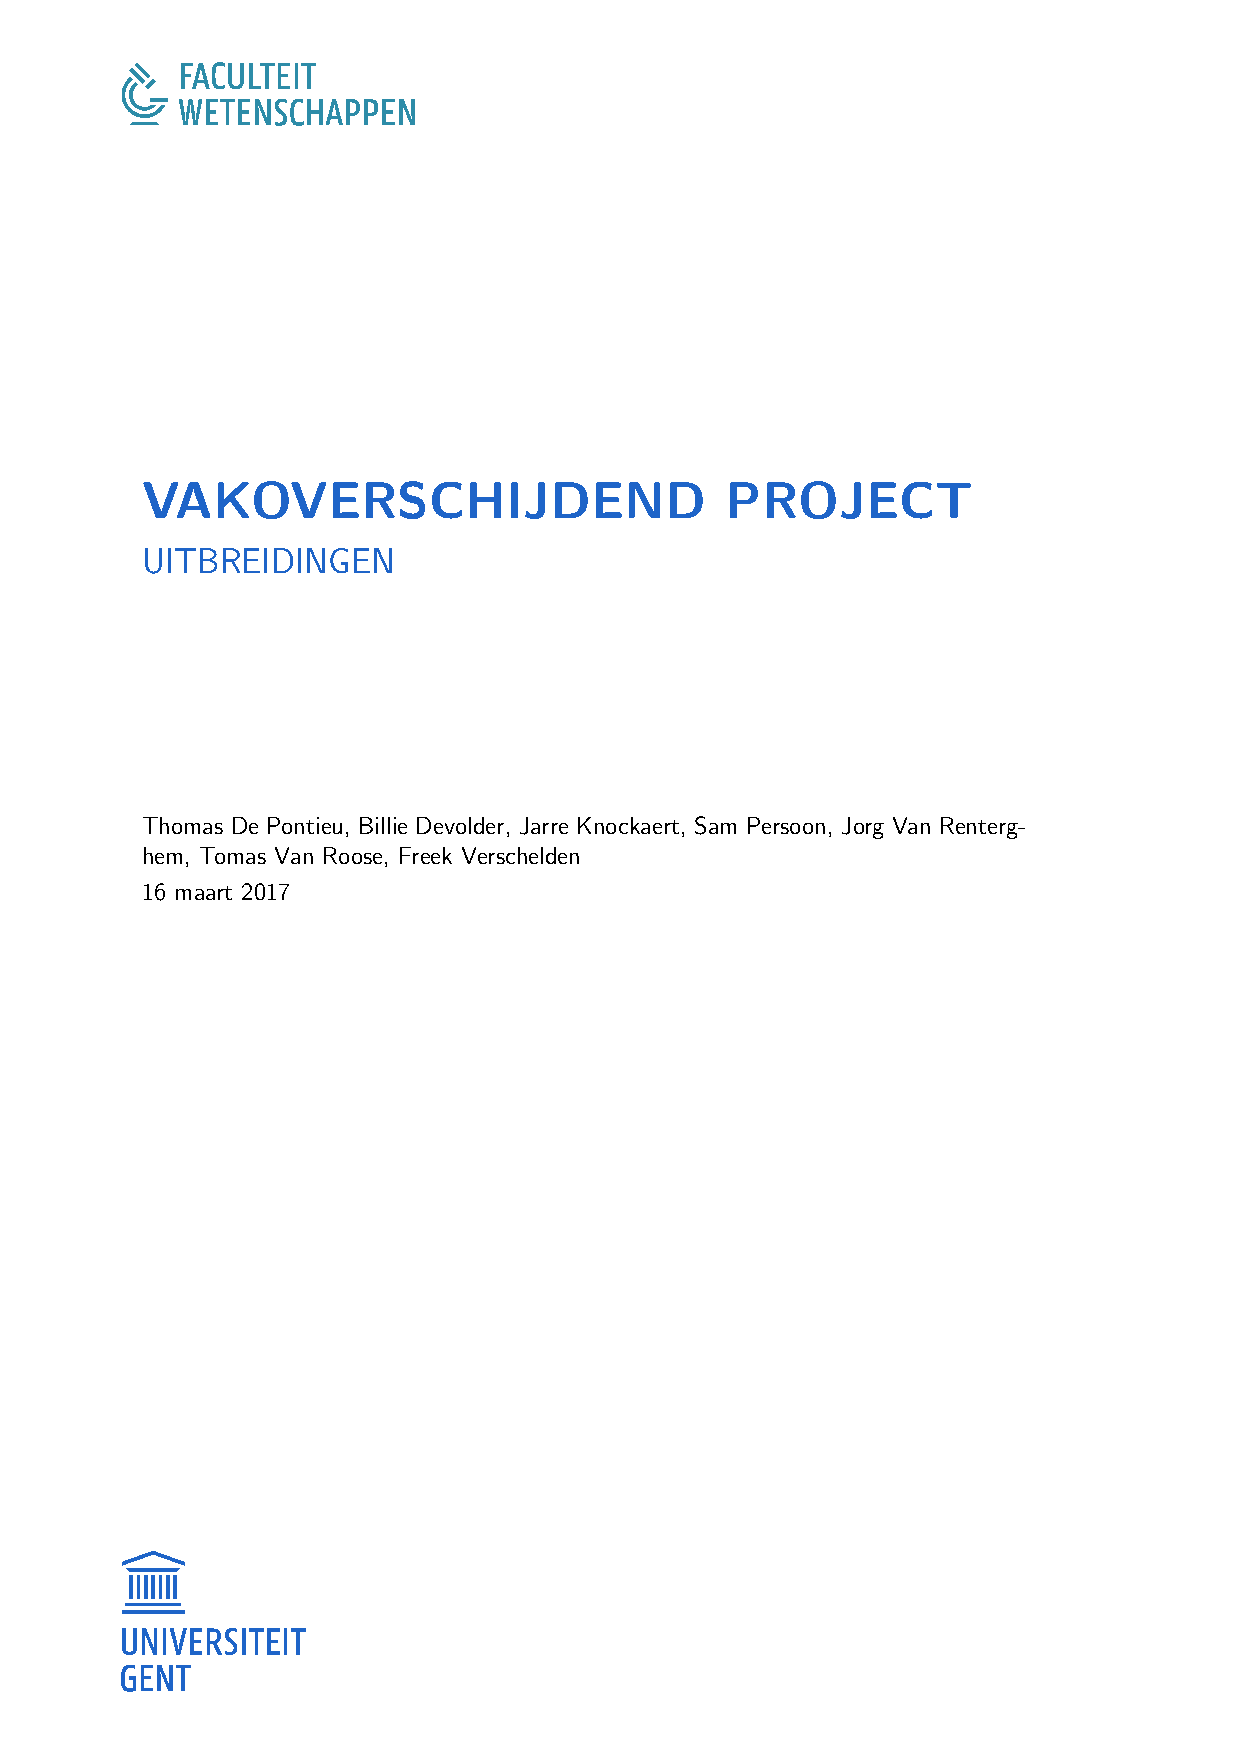
\includepdf[pages={1}]{voorblad.pdf}
\section{Vloten samenvoegen}

De eerste uitbreiding die we zullen bespreken is het samenvloegen van vloten. Indien 2 vestigingen van een bedrijf fuseren en de vloten moeten worden samengevoegd, zou het handig zijn dit met een simpele druk op een knop te kunnen doen. In principe moet er voor deze uitbreiding niets worden veranderd in de backend. De frontend kan alle voertuigen van een bepaalde vloot opvragen en dan via een PUT request de vloot veranderen van alle voertuigen in de vloot.
\\
\\
De aanpassingen staan hier zeker in verhouding tot de uitbreiding. In de backend en database moet er namelijk niets aangepast worden.

\section{Ondersteunen van boten}
	
Misschien wil Solvas, in een verre toekomst, zich ook gaan bezighouden met het verzekeren van boten. Hier nemen we aan dat het verzekeren van boten gebeurt op een gelijkaardige manier.
\\
\\
In het domeinmodel zou er een nieuwe klasse, \verb|WaterCraft|, moeten toegevoegd worden. Deze klasse zou een boot voorstellen en sterk lijken op de huidige klasse \verb|Vehicle|. Deze 2 klassen zouden grote gelijkenissen vertonen dus zou hier best een gemeenschappelijke superklasse voor gemaakt worden. In dit document zal deze superklasse \verb|AbstractVehicle| worden genoemd. De klasse \verb|Fleet| zou dan ook een collectie \verb|AbstractVehicle| objecten moeten hebben in plaats van \verb|Vehicle| objecten.
\\
\\
In de andere lagen zou er een \verb|DataAccessObject|, een \verb|Controller| en een \verb|RESTController| moeten bijkomen specifiek voor boten. \verb|WaterCraftDAO| en \verb|WaterCraftController| zouden dan overerven van respectievelijk \verb|DAO| en \verb|AbstractController| zodat enkel de update en create methodes nog moeten worden geïmplementeerd. Aan de klasse \verb|DAOProvider| zou er een methode moeten worden toegevoegd zodat de nieuwe \verb|DAO| kan worden opgevraagd. 
\\
\\
We denken dat de aanpassingen in verhouding staan tot de uitbreiding. Het meeste werk zou kruipen in het doorgeven van de waarden van de velden en deze te setten in de objecten. Dit is repetitief werk maar niet iets dat gemakkelijk te veralgemenen is. De meeste veranderingen in het domeinmodel zijn eenmalig. Indien er nog een ander soort voertuig zou bijkomen met andere velden, zou er enkel een klasse moeten worden toegevoegd die overerft van \verb|AbstractVehicle|.
\end{document}
